\section{Qualitätssicherung (Testprotokoll)}

	\subsection{Registrieren Sie sich.}
	Verwenden Sie:
	\begin{itemize}
		\item E-Mail: [vorname].mail.de
		\item Passwort: 123456 
	\end{itemize}
	\ \\
	\begin{tabular}{|>{$\rhd$ }lrl|}
		\hline
		Sehr gut  & \mybar{10}\\
		gut  & \mybar{5}\\
		ok               & \mybar{3}\\
		schlecht         & \mybar{4}\\
		\hline
	\end{tabular}
	
	\subsection{Melden Sie sich mit Ihren Nutzerdaten an.}
	\begin{tabular}{|>{$\rhd$ }lrl|}
		\hline
		Sehr gut  & \mybar{10}\\
		gut  & \mybar{5}\\
		ok               & \mybar{3}\\
		schlecht         & \mybar{4}\\
		\hline
	\end{tabular}
	
	\subsection{Erstellen Sie eine Reise.}
	\begin{tabular}{|>{$\rhd$ }lrl|}
		\hline
		Sehr gut  & \mybar{10}\\
		gut  & \mybar{5}\\
		ok               & \mybar{3}\\
		schlecht         & \mybar{4}\\
		\hline
	\end{tabular}
	
	\subsection{Öffnen Sie die Einladungsseite ihrer Reise.}
	\begin{tabular}{|>{$\rhd$ }lrl|}
		\hline
		Sehr gut  & \mybar{10}\\
		gut  & \mybar{5}\\
		ok               & \mybar{3}\\
		schlecht         & \mybar{4}\\
		\hline
	\end{tabular}
	
	\subsection{Versuchen Sie einer Reise beizutreten, wenn Ihnen folgendes Bild geschickt wurde: (sieh Abb. \ref{fig:user_test_invite}).}
	\begin{tabular}{|>{$\rhd$ }lrl|}
		\hline
		Sehr gut  & \mybar{10}\\
		gut  & \mybar{5}\\
		ok               & \mybar{3}\\
		schlecht         & \mybar{4}\\
		\hline
	\end{tabular}
	
	\begin{figure}[H]
	\centering
	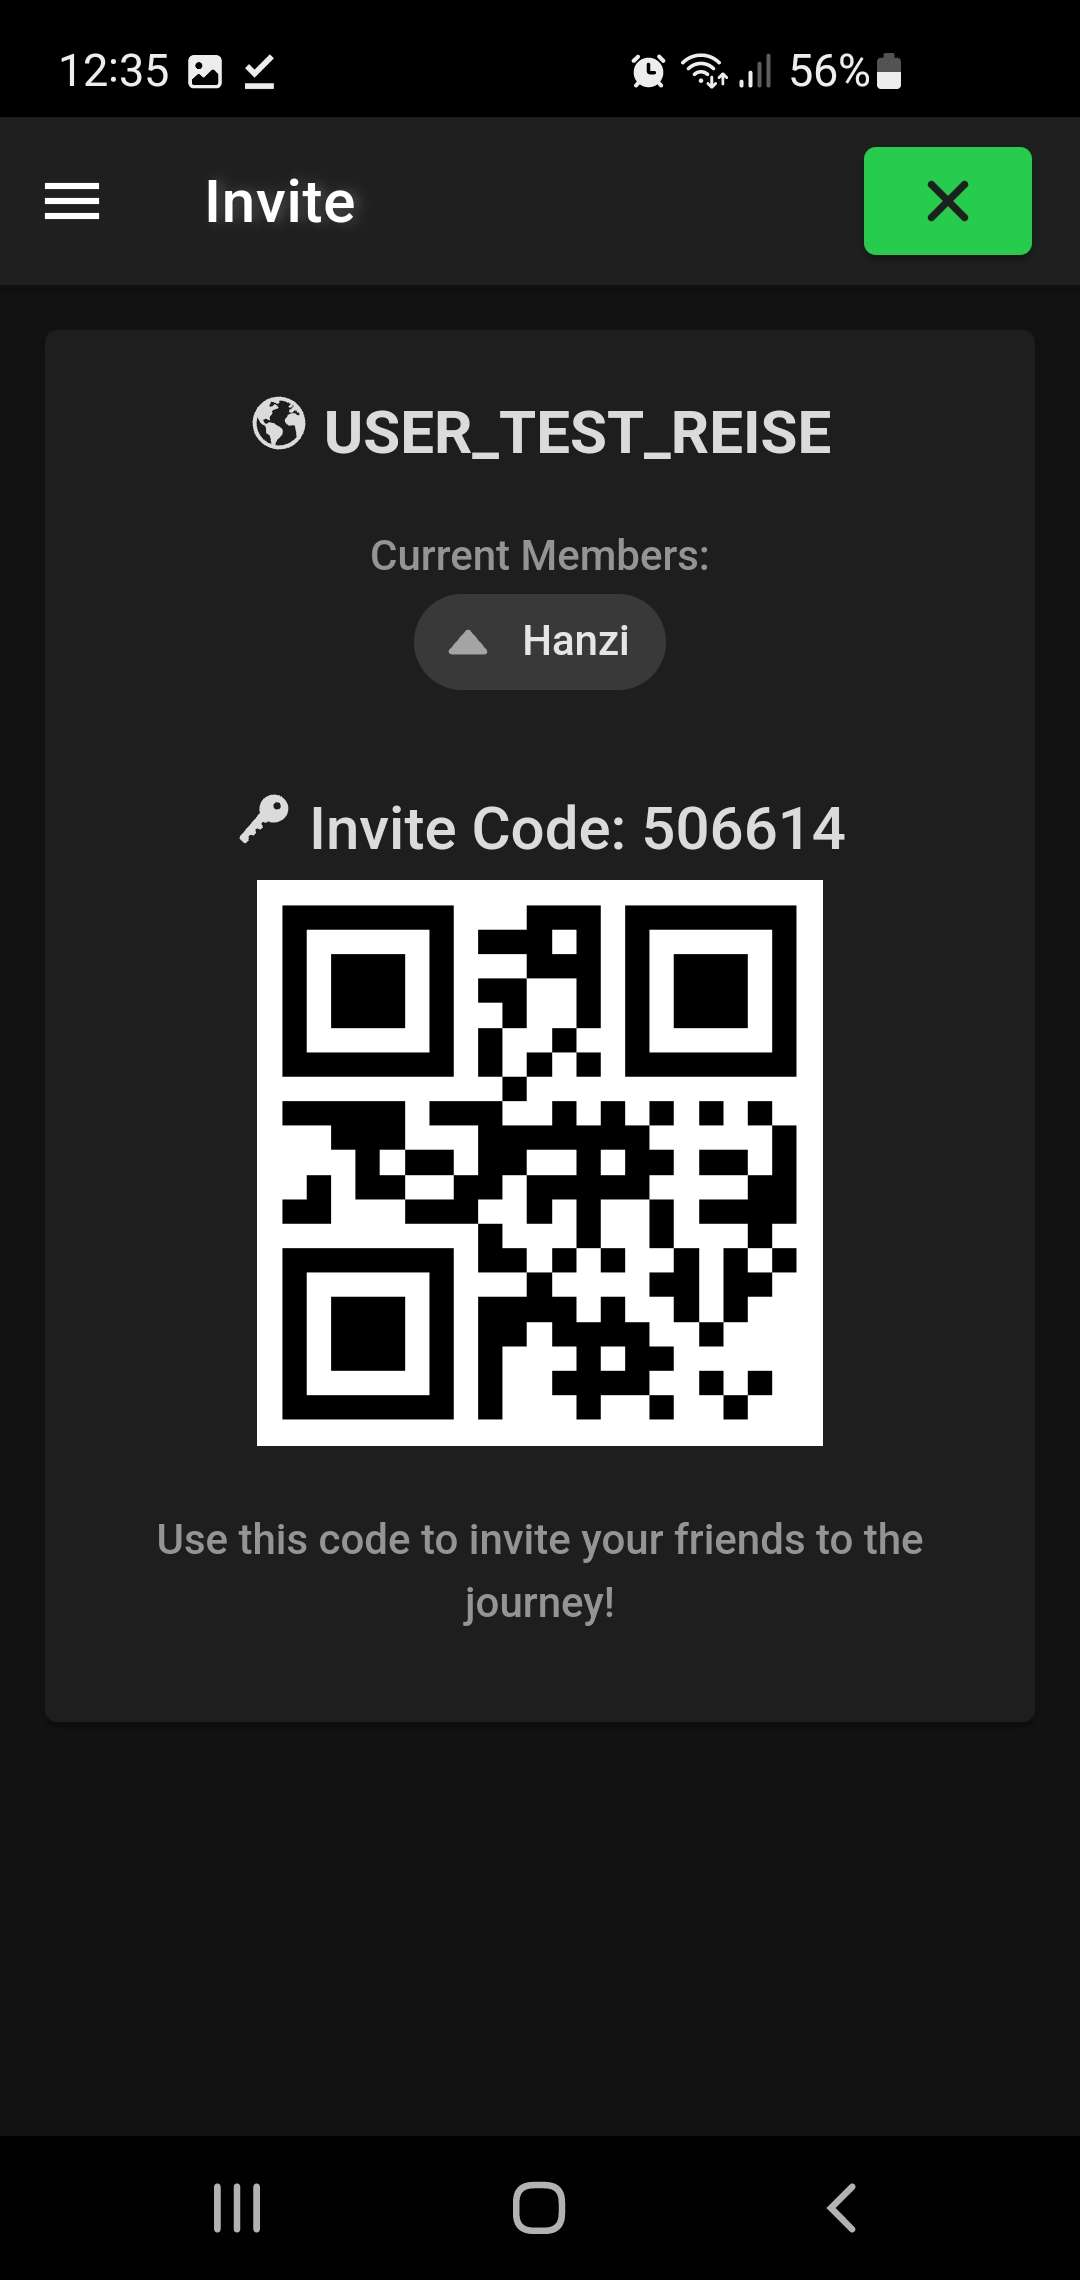
\includegraphics[width=0.3
		\textwidth]{img/user_test_invite}
	\caption[Usertest Einladung]{Usertesteinladung}
	%\captionsource{}
	\label{fig:user_test_invite}
\end{figure}

	\subsection{Erstellen Sie in der Reise 'User\_Test\_Reise' eine Ausgabe, bei der Sie 50 € für ein Mittagessen mit Hanz und Maria gezahlt haben.}
	\begin{tabular}{|>{$\rhd$ }lrl|}
		\hline
		Sehr gut  & \mybar{10}\\
		gut  & \mybar{5}\\
		ok               & \mybar{3}\\
		schlecht         & \mybar{4}\\
		\hline
	\end{tabular}
	
	\subsection{Bearbeite Sie die Zahlung zu 85 €.}
	\begin{tabular}{|>{$\rhd$ }lrl|}
		\hline
		Sehr gut  & \mybar{10}\\
		gut  & \mybar{5}\\
		ok               & \mybar{3}\\
		schlecht         & \mybar{4}\\
		\hline
	\end{tabular}
	
	\subsection{Lassen Sie sich die Schulden der Reise anzeigen.}
	\begin{tabular}{|>{$\rhd$ }lrl|}
		\hline
		Sehr gut  & \mybar{10}\\
		gut  & \mybar{5}\\
		ok               & \mybar{3}\\
		schlecht         & \mybar{4}\\
		\hline
	\end{tabular}
	
	\subsection{Vermerken Sie, dass Maria 5 € zurückgezahlt hat.}
	\begin{tabular}{|>{$\rhd$ }lrl|}
		\hline
		Sehr gut  & \mybar{10}\\
		gut  & \mybar{5}\\
		ok               & \mybar{3}\\
		schlecht         & \mybar{4}\\
		\hline
	\end{tabular}
	
	\subsection{Erstellen Sie in der Reise 'User\_Test\_Reise' eine Ausgabe bei der Hanz für Sie beide ein Taxi am 03.01.23 für 100 € gezahlt hat.}
	\begin{tabular}{|>{$\rhd$ }lrl|}
		\hline
		Sehr gut  & \mybar{10}\\
		gut  & \mybar{5}\\
		ok               & \mybar{3}\\
		schlecht         & \mybar{4}\\
		\hline
	\end{tabular}
	
	\subsection{Lassen Sie sich die Schulden der Reise erneut anzeigen. Ändern Sie die Währung zu £.}
	\begin{tabular}{|>{$\rhd$ }lrl|}
		\hline
		Sehr gut  & \mybar{10}\\
		gut  & \mybar{5}\\
		ok               & \mybar{3}\\
		schlecht         & \mybar{4}\\
		\hline
	\end{tabular}
	
	\subsection{Halten Sie fest, dass Sie Hanz die Schulden zurückgezahlt haben.}
	\begin{tabular}{|>{$\rhd$ }lrl|}
		\hline
		Sehr gut  & \mybar{10}\\
		gut  & \mybar{5}\\
		ok               & \mybar{3}\\
		schlecht         & \mybar{4}\\
		\hline
	\end{tabular}
	
	\subsection{Ändern Sie die Sortierung für die Ausgaben der Reise 'User\_Test\_Reise'.}
	\begin{tabular}{|>{$\rhd$ }lrl|}
		\hline
		Sehr gut  & \mybar{10}\\
		gut  & \mybar{5}\\
		ok               & \mybar{3}\\
		schlecht         & \mybar{4}\\
		\hline
	\end{tabular}
	
	\subsection{Löschen Sie alle Ausgaben der Reise 'User\_Test\_Reise'.}
	\begin{tabular}{|>{$\rhd$ }lrl|}
		\hline
		Sehr gut  & \mybar{10}\\
		gut  & \mybar{5}\\
		ok               & \mybar{3}\\
		schlecht         & \mybar{4}\\
		\hline
	\end{tabular}
	
	\subsection{Archivieren Sie die von Ihnen erstellte Reise.}
	\begin{tabular}{|>{$\rhd$ }lrl|}
		\hline
		Sehr gut  & \mybar{10}\\
		gut  & \mybar{5}\\
		ok               & \mybar{3}\\
		schlecht         & \mybar{4}\\
		\hline
	\end{tabular}
	
	\subsection{Loggen Sie sich aus der App aus.}
	\begin{tabular}{|>{$\rhd$ }lrl|}
		\hline
		Sehr gut  & \mybar{10}\\
		gut  & \mybar{5}\\
		ok               & \mybar{3}\\
		schlecht         & \mybar{4}\\
		\hline
	\end{tabular}